\documentclass{scrartcl}
\usepackage{selinput}
\SelectInputMappings{
  adieresis={ä},
  germandbls={ß},
}
\usepackage[ngerman]{babel}

\usepackage{graphicx}
\usepackage[hidelinks]{hyperref}
\usepackage{csquotes}
\MakeOuterQuote{"}
\usepackage{biblatex}

\usepackage{amsmath}
\usepackage{amssymb}

\usepackage{dirtree}
\usepackage{tabularx}

\bibliography{quellen}

\begin{document}

\titlehead{
  Universität Leipzig \\
  Fakultät für Mathematik und Informatik \\
  Institut für Informatik
}
\subject{Projekt Dokumentation}
\title{Generische Methoden für das Faktorisieren und die Berechnung diskreter Logarithmen}
%\subtitle{}
\author{Schindler, Benjamin \and Schmierer, Lukas}
\date{\today}
\publishers{Dr. Claus Diem}
\maketitle

\tableofcontents

\section{Problemstellung}
Diese Projektarbeit, entstanden im Rahmen des Moduls "Mathematische Grundlagen der Kryptographie mit öffentlichen Schlüsseln", beschäftigt sich dem Lösen diskreter Logarithmen und dem Faktorisieren. Wir verwenden dazu sogenannte \emph{generische Methoden}. Diese verwenden ausschließlich allgemeine Gruppeneigenschaften ohne auf die Struktur der zugrundeliegenden Gruppe einzugehen. Es sind zwar asymptotisch schnellere Algorithmen zum lösen des diskreten Logarithmus und zur Faktorisierung bekannt \cite{diem_2011, Adleman_1979}[noch mehr Quellennachweise], jedoch können die hier vorgestellten Algorithmen auf allen endlichen zyklischen Gruppen angewendet werden. In unserem Projekt arbeiten wir mit Restklassenkörpern, Polynomrestklassenkörpern und darauf aufbauende elliptische Kurven in unterschiedlichen Darstellungen. Die dazu benötigten Grundlagen sind in \cite{Galbraith2012} ausführlich beschrieben. 
\section{Projekt Organisation}
\label{sec:organisation}

\subsection{Verzeichnisstruktur}
\label{sec:verzeichnisstruktur}
Eine Schematische Darstellung der Verzeichnisstruktur ist in Abbildung \ref{fig:verzeichnisstruktur} zu sehen.\\
In unserem Projekt befinden sich drei Verzeichnisse:

\begin{itemize}
\item \emph{tocas} - Enthält den von Dr. Claus Diem bereitgestellten Python Code aus \emph{Tocas} \cite{tocas} unverändert.

\item \emph{ha} - Abkürzung für \emph{Hausaufgaben}. Enthält unsere Python Implementierung zur Lösung der Hausaufgaben aus der Vorlesung "Mathematische Grundlagen der Kryptographie mit öffentlichen Schlüsseln"
\item \emph{projekt} - Enthält den im Rahmen unserer Projektarbeit geschriebenen Python Code zur Lösung des Diskreten Logarithmus Problems und zur Faktorisierung mithilfe generischer Methoden.
\end{itemize}
Da das \emph{tocas}-Projekt separat vorliegt, können dadurch zukünftige Änderungen und Updates in unser Projekt eingepflegt werden. Außerdem erreichen wir so eine strikte Trennung von bereitgestelltem und eigenem Code.\\
Wenn zu bereits existierenden Klassen aus \emph{Tocas} weitere Funktionalitäten hinzugefügt wurden, wurden diese in externe Module geschrieben, die den Datei-Suffix \emph{\_extension} tragen. So verschönert zum Beispiel das Modul \emph{'format\_extension.py'} die Standard-Ausgabe von Tocas (z.B. die Ausgabe für den Ring der ganzen Zahlen mit \( \mathbb{Z} \) statt Z). \\
Innerhalb der Ordner \emph{ha} und \emph{project} befindet sich jeweils ein Unterordner \emph{tests}. In diesem sind verschiedene Tests geschrieben, die mit der Web-Applikation \emph{Jupyter Notebook} aus \cite{jupyterNotebook} ausgeführt werden können.

\begin{figure}[h]
  \fbox{
    \begin{minipage}{0.9\textwidth}
    \dirtree{%
    .1 projekt\_generisches\_faktorisieren\_und\_dlp.
    .2 tocas.
    .3 ....
    .2 ha.
    .3 tests.
    .4 ....
    .3 format\_extension.py.
    .3 ....
    .2 projekt.
    .3 tests.
    .4 ....
    .3 ....
    .2 dokumentation.pdf.
    }
    \end{minipage}
  }
  \caption{Verzeichnisstruktur des Projekts}
  \label{fig:verzeichnisstruktur}
\end{figure}

\subsection{Tests}
\label{sec:tests}

Zu jedem Teilgebiet wurden zugehörige Tests als Jupyter Notebooks erstellt. Dabei gibt der Name des Tests an, welche Funktionalität getestet wird. Eine Liste aller Tests die wir im Rahmen unserer Projektarbeit geschrieben haben sind inklusive einer kurzen Beschreibung in Tabelle \ref{tab:tests} zu sehen.
\begin{table}[!ht]
\centering
\begin{tabularx}{\linewidth}{X|p{8.8cm}}
  \begin{minipage}{\linewidth}
      \emph{test\_edwards\_kurven.ipynb} \\
      \emph{test\_weierstrass\_kurven.ipynb}
  \end{minipage} &
  \begin{minipage}{\linewidth}
        \vspace{2pt} Testet grundlegende Funktionalität unserer Realisierung Elliptischer Kurven über endlichen Körpern in den Darstellungen nach Edwards und Weierstrass. \vspace{2pt}
  \end{minipage} \\
  \hline
  \begin{minipage}{\linewidth}
      \emph{test\_pohlig\_hellman.ipynb}
  \end{minipage} &
  \begin{minipage}{\linewidth}
      \vspace{2pt} Testet das Verfahren nach Pohlig und Hellman zur Reduktion endlicher Gruppen in zyklische Untergruppen. 
      Dabei werden auch verschiedene Verfahren zur anschließenden Berechnung  des diskreten Logarithmus ausgeführt.   \vspace{2pt}
  \end{minipage} \\
  \hline
    \begin{minipage}{\linewidth}
    \emph{test\_baby\_step\_giant\_step.ipynb} \\
    \emph{test\_rho.ipynb}  \\
    \emph{test\_kaenguru.ipynb} 
  \end{minipage} &
  \begin{minipage}{\linewidth}
    \vspace{2pt} Testet die von uns implementierten Methoden zu Berechnung des diskreten Logarithmus. Neben dem Baby-Step-Giant-Step-Algorithmus und dem Känguru-Algorithmus (auch Lambda-Methode genannt) 
    werden verschiedene Varianten des Rho-Algorithmus ausgeführt  \vspace{2pt}
  \end{minipage} \\
  \hline
    \begin{minipage}{\linewidth}
    \emph{test\_rho\_faktorisieren.ipynb}
  \end{minipage} &
  \begin{minipage}{\linewidth}
      \vspace{2pt} Testet die Rho-Methode zur Faktorisierung ganzer Zahlen.   \vspace{2pt}
  \end{minipage}
\end{tabularx}
\renewcommand{\arraystretch}{1}
\caption{Übersicht der Jupyter Notebook Tests unserer Projektarbeit}
\label{tab:tests}
\end{table}


\section{Implementierung}
\label{sec:implementierung}

\subsection{Elliptische Kurven}
\label{sec:elliptische_kurven}

Um zu zeigen, dass unsere generischen Methoden auf verschiedenste Gruppen anwendbar sind, mussten neben den bereits implementieren endlichen Körpern zusätzlich auch elliptische Kurven über endliche Körper realisiert werden. 
Die in \emph{abstrakte\_gruppen.py} eingeführten Klassen \emph{AdditiveGruppe} und \emph{AdditiveGruppenElement} dienen als Basisklassen unserer elliptischen Kurvengruppen.
Anschließend haben wir uns 2 verschiedenen Darstellungen Elliptischer Kurven bedient, der Edwards-Darstellung und der kurzen Weierstraß-Darstellung. Diese sind beispielsweise in \cite{Galbraith2012} ausführlich beschrieben. In den nachfolgenden Kapiteln werden sie noch einmal kurz vorgestellt.

\subsubsection{Edwards-Darstellung}
\label{sec:edwards_kurven}
Sei $\mathbb{F}_q$ ein endlicher Körper.
Eine elliptische Kurve über $\mathbb{F}_q$ in Edwards-Darstellung erfüllt folgende Formel:
$$ x^2+y^2= 1+dx^2y^2$$
mit den affinen Koordinaten $x,y \in \mathbb{F}_q$ und dem Parameter $d \in \mathbb{F}_q$.
Desweiteren gelten folgende Formeln: \vspace{5pt}\\
Die Addition \ $(x_1,y_1)+(x_2,y_2)=(x_3,y_3)$\quad mit: \\
\begin{align*}
  &x_3=\frac{x_1y_2 + x_2 y_1} { 1 + d x_1 x_2  y_1y_2}
  &y_3=\frac{y_1 y_2 - x_1 x_2}{1 - d x_1  x_2 y_1  y_2}
\end{align*}\\
und die Negation: \ $-(x_1,x_2)=(-x_1,y_1) $ \vspace{5pt} \\
Daraus ergibt sich das Neutrale Element  $(0, 1)$\\
Die obigen Berechnungsvorschriften wurden in der Klasse  \emph{EdwardsKurvengruppenElement} implementiert.
\subsubsection{kurze Weierstraß-Darstellung}
\label{sec:weierstrass_kurven}
Sei $\mathbb{F}_q$ ein endlicher Körper.
Eine elliptische Kurve über $\mathbb{F}_q$ in kurzer Weierstraß Darstellung und affiner Schreibweise erfüllt folgende Formel:
$$ y^2 = x^3 + ax +b$$
mit den affinen Koordinaten $x,y \in \mathbb{F}_q$ und den Parametern $a, b \in \mathbb{F}_q$.
Desweiteren gelten folgende Formeln: \vspace{5pt}\\
Die Addition \ $(x_1,y_1)+(x_2,y_2)=(x_3,y_3)$\quad mit: \\
\begin{align*}
 %\begin{split}
  &x_3=\frac{(y_1-y_2)^2}{(x_1-x_2)^2}-x_1-x_2
  &y_3=\frac{(y_1-y_2)}{(x_1-x_2)}\cdot (x_1 - x_3) - y_1
 %\end{split}
\end{align*}\\
das Verdoppeln \ $ 2(x_1,y_1)=(x_3,y_3) $\quad mit: \\
\begin{align*} 
  &x_3=\frac{(3x_1^2+a)^2}{4y_1^2}-2x_1
  &y_3= \frac{3x_1^2+a}{2y_1} \cdot (x_1 - x_3) - y_1
\end{align*}\\
und die Negation: \ $-(x_1,x_2)=(x_1,-y_1) $ \vspace{5pt} \\
Die obigen Berechnungsvorschriften wurden in der Klasse \emph{WeierstrassKurvengruppenElement} implementiert. Das neutrale Element der Gruppe ist der sogenannte \emph{Punkt im Unendlichen} der in affiner Schreibweise nicht dargestellt werden kann. Deshalb verwenden wir in unserer Implementierung des Gruppenelementes ein Attribut {\emph{isPointAtInfinity}}, welches angibt, ob es sich bei dem Punkt um das neutrale Element handelt. Bei jeder Addition und Verdopplung wird dieses Attribut abgefragt und die entsprechende Berechnung übersprungen.
\subsection{Pohlig-Hellman Reduktion}
\label{sec:pohlig_hellman}
Die Reduktion nach Pohlig und Hellman zur Lösung des diskreten Logarithmus wurde zum ersten mal in \cite{Pohlig1978} eingeführt. Unsere Implementation befindet sich im Modul \emph{pohlig\_hellman}. In dem Verfahren wird die ursprüngliche Gruppe in deren zyklischen Untergruppen zerlegt. Anschließend wird versucht den diskreten Logarithmus in den kleineren Untergruppen zu berechnen, um anschließend mittels chinesischem Restklassensatz die Lösung in unserer ursprünglichen Gruppe zu berechnen. Dazu muss die Faktorisierung der Gruppenordnung bekannt sein und als Funktionsparameter übergeben werden. Der Algorithmus arbeitet nur dann wirklich effektiv, wenn die Gruppenordnung aus möglichst kleinen Primfaktoren besteht.\\
Der Algorithmus zur Berechnung des diskreten Logarithmus in den Untergruppen ist in unserer Implementation modular austauschbarer und wird als Funktionsparameter übergeben (Standard ist die erschöpfende Suche). Es können also alle hier vorgestellten Algorithmen verwendet werden.
\subsection{Baby-Step Giant-Step}
\label{sec:baby_step_giant_step}
Der Baby-Step Giant-Step Algorithmus ist eine Modifikation des naiven Algorithmus zur Lösung des diskreten Logarithmus  \cite{Galbraith2012}. Dabei beschleunigen wir die Suche, indem wir Zwischenergebnisse effizient abspeichern. Dazu verwenden wir Pythons native \emph{Dictionary}-Datenstruktur. Dabei handelt es sich um eine Hash-Tabelle. Die schnellen Lesezugriffen ermöglichen eine effiziente Überprüfung, ob sich ein Element bereits in unserer Hash-Tabelle befindet.
\subsection{Rho Methode}
\label{sec:rho}
Die \emph{Rho}-Methode von Pollard hat im Vergleich zum Baby-Step Giant-Step Algorithmus den Vorteil,
dass sie deutlich weniger Speicherplatz benötigt.
Dadurch eignet sie sich besser für die Berechnung des DLP auf aktueller Computer-Hardware.

Die \emph{Rho}-Methoden basieren auf sogenannten \emph{pseudorandom walks}.
Sie bestehen prinzipiell aus einem Algorthmus zur Zyklussuche
und einer Walk Funktion.
Die Zyklussuche ist generisch über die Walk Funktion.

Es wurden verschiedene Zyklussuchen und Walk Funktion
implementiert.
Dabei haben wir uns an den Ausführungen in \cite{Galbraith2012}
orientiert.
Unsere Implementierungen sind in der Datei \emph{rho.py} zu finden.

\subsubsection{Walk Funktion}
\label{sec:walk_funktion}
Es wurden zwei verschiende \emph{walk}-Funktionen implementiert.
Diese sind Pollards originaler rho walk und Pollards additiver rho walk.
Beide Methoden sind sich in ihrer Charakteristik allerdings sehr ähnlich.

Die Schrittgrößen werden jeweils zu Beginn pseudozufällig bestimmt.
Dadurch benötigt jeder Schritt später immer nur eine Gruppenoperation.

Alle Zyklussuch-Methoden können mit beiden Walk Funktionen genutzt werden.
Das wurde erreicht, indem die Walk Funktion als Funktion übergeben werden kann.

\subsubsection{Floyd Cycle}
\label{sec:floyd_cycle}
In der originalen Ausführung des Rho Algorithmus nutztz Pollard
den \emph{Floyd Cycle} Algorithmus zur Zyklussuche.
Bei dieser laufen zwei pseudorandom Walks jeweils bei 0 und 1 los,
wobei einer doppelt so schnell läuft wie der andere.
Wenn eine Kolision gefunden wurde, ist das DLP gelöst.

Die \emph{Floyd Cycle} Suche ist nicht besonders effizient.
Im Durchschnitt benötigt sie \( 2.47(l_t + l_h) \) Operationen.
\( l_t \) ist hierbei die Länge des Schwanzes und \( l_h \) die
Länge des Zyklus.
\cite{Galbraith2012}

\subsubsection{Brent Cycle}
\label{sec:brent_cycle}
Als eine effizientere Methode im Vergleich zur Floyd Cycle Suche
haben wir die Zyklussuche nach Brent \cite{Brent1980} implementiert.
Bei dieser Methode müssen wie bei der Floyd Suche nur zwei Elemente gespeichert werden.
\cite{Galbraith2012}

Brent führt in seiner Veröffentlichung theoretisch aus warum, warum seine
Zyklussuche im allgemeinen Fall schneller ist.
Dabei zeigt er einen Laufzeitvorteil von 36 Prozent.
\cite{Brent1980}

\subsubsection{Distinguished Points}
\label{sec:distinguished_points}
Die effizienteste Methode die wir implementiert haben ist die
\emph{distinguished points} Methode.
Bei dieser Methode werden bestimmte Zahlen als "besonders" gekennzeichnet.
Welche Zahlen dies sind ist prinzipiell willkürlich.
Wir haben dabei Zahlen gewählt deren letzen \emph{n} Stellen in einer
zwei adischen Darstellung 0 sind.

Bei der distinguished points Methode wird von einer zufälligen Zahl aus
der Walk gestartet und dann beedenet wenn ein "besonderer" Punkt
gefunden wurde.
Dies wird so lange wiederholt bis der gleiche Punkt zweimal gefunden wurde.

Während die beiden zuerst vorgestellten Methoden immer nur zwei Punkt abspeichern müssen,
muss bei der distinguished points Methode jeder gefundene "besondere" Punkt gespeichert werden.
Der Speicheraufwand ist allerdings trozdem noch bei weitem geringer als beispielsweise beim
Baby-Step Giant-Step Algorithmus.
\cite{VanOorschot1999}

\subsection{Känguru Methode}
\label{sec:kaenguru}
Eine weitere Methode die auf pseudorandom Wals basiert ist die
\emph{Känguru} oder \(\lambda\)-Methode.
Während die Känguru Methode im allgemeinen langsamer als die Rho
Methode mit distinguished points ist, hat sie einen weiteren Anwendungsfall.
Mit ihr lässt sich der diskrete Logarithmus sehr effizient berechnen,
wenn vorher bekannt ist, dass er in einem bestimmten Bereich liegt.

Bei der Känguru Methode ist die Walk Funktion im Vergleich zur Rho Methode
komplett deterministisch und nicht pseudorandom.
Unsere Implementierung arbeitet auch mit distinguished points und ist in
der Datei \emph{kaenguru.py} zu finden.
\cite{Galbraith2012}

\subsection{Vergleich zwischen Rho Methoden und Känguru Methode}
Um die theoretischen Annahmen über die Laufzeit der verschiedenen Methoden
zu validieren, wurden Laufzeitmessungen durchgeführt.
Dabei wurde der diskrete Logarithmus \( a = 2778286 \) zu \( g = 3805914789 \)
und \(h = g^a = 2262438373 \) in \( \mathbb{F}_{32416190071} \) gesucht.
Jede Messung wurde 10 mal durchgeführt und die Messwerte anschließend gemittelt.
Die Messergebnisse sind in Tabelle \ref{tab:benchmark} dargestellt und
in Abbildung \ref{fig:benchmark} als Boxplot visualisiert.

\begin{table}[h]
  \centering
  \begin{tabular}{l|c|c|c}
    Methode             & min   & max   & avg   \\ \hline
    Rho (Floyd)         & 1,020 & 2,608 & 1,897  \\ \hline
    Rho (Brent)         & 0,838 & 3,525 & 1,880 \\ \hline
    Rho (Distinguished) & 0,776 & 2,149 & 1,281 \\ \hline
    Känguru             & 1,922 & 1,936 & 1,929
    \end{tabular}
  \caption{Laufzeit verschiedener Rho Methoden und der Känguru Methode in Sekunden}
  \label{tab:benchmark}
\end{table}

\begin{figure}[h]
  \centering
  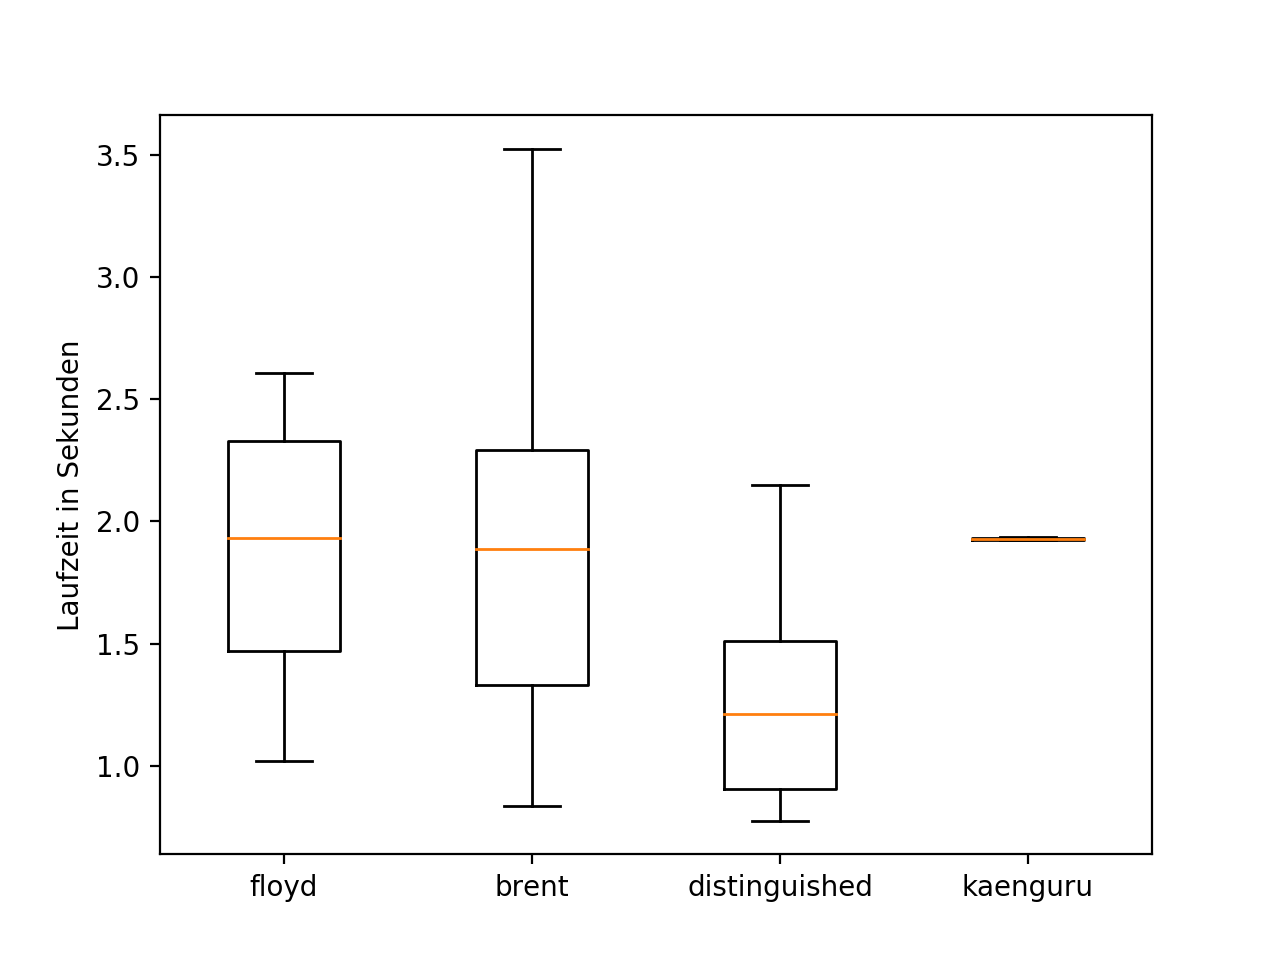
\includegraphics[width=0.6\textwidth]{../projekt/benchmark/plot_dlp.png}
  \caption{Grafische Darstellung der Laufzeit verschiedener Rho Methoden und der Känguru Methode}
  \label{fig:benchmark}
\end{figure}

Die Laufzeiten der verschiedenen Methoden verhalten sich gemäß der
theoretischen Erwartungen aus \ref{sec:floyd_cycle},
\ref{sec:brent_cycle}, \ref{sec:distinguished_points} und
\ref{sec:kaenguru}.
Die \emph{Rho} Methode ist der \emph{Kängeru} Methode überlegen,
wobei die Zyklus Suche mit \emph{Distinguished Points} die durchschnittlich
kürzeste Laufzeit aufweist.

Es lässt sich beobachten, dass die Laufzeitmessungen der \emph{Känguru}
Methode im Vergleich zu den anderen \emph{Rho} Methoden eine geringe Varianz
aufweisen.
Dies lässt sich damit erklären, dass die \emph{walk}-Funktion der
\emph{Känguru} Methode in unserer Implementierung keine zufälligen
Schrittgrößen nutzt und der Algorithmus somit komplett deterministisch
ist.

\subsection{Parallelisierung der Rho-Methode}

Um eine bessere Laufzeit zu erhalten, wurde die \emph{Rho}-Methode in der distinguished points Variante parallelisiert. 
Die Implementierung ist in \emph{parallel\_rho.py} zu finden. \\
Es wurde der diskrete Logarithmus \( a = 67782867 \) zu \( g = 1580023 \)
und \(h = g^a = 541805201268 \) in \( \mathbb{F}_{1624571841187} \) berechnet.\\
Alle Berechnungen wurden auf dem Rechenserver \emph{miserv100} der Universität Leipzig ausgeführt ($12$ Kerne mit $3.07$ GHz, $196$ GB RAM).
Dabei wurden verschiedene Parallelisierungsgrade mit bis zu 10 Threads verwendet. 
Die Berechnungen wurden 10 mal wiederholt. Die Ergebnisse sind in Tabelle \ref{tab:benchmark:parallel} dargestellt und in Abbildung \ref{fig:benchmark:parallel} als Boxplot visualisiert. \\
Es ist eine deutliche Beschleunigung der Laufzeit durch die Parallelisierung zu beobachten.
\begin{table}[h]
  \centering
  \begin{tabular}{l|c|c|c}
    Methode             & min   & max   & avg   \\ \hline
    Rho (Distinguished) & 10.170 & 135.699 & 63.174 \\ \hline
    Rho (parallel, 2 Threads) & 8.703 & 118.479 & 50.924 \\ \hline
    Rho (parallel, 4 Threads) & 7.530 & 31.715 & 17.006 \\ \hline
    Rho (parallel, 6 Threads) & 5.492 & 28.699 & 14.579 \\ \hline
    Rho (parallel, 8 Threads) & 3.135 & 21.540 & 10.070 \\ \hline
    Rho (parallel, 10 Threads) & 3.413 & 19.295 & 11.619 \\ \hline
    \end{tabular}
  \caption{Laufzeit der Rho-Methode in der Distinguished-Points-Variante ohne Parallelisierung, sowie parallelisiert mit 6 und 11 Threads in Sekunden}
  \label{tab:benchmark:parallel}
\end{table}

\begin{figure}[h]
  \centering
  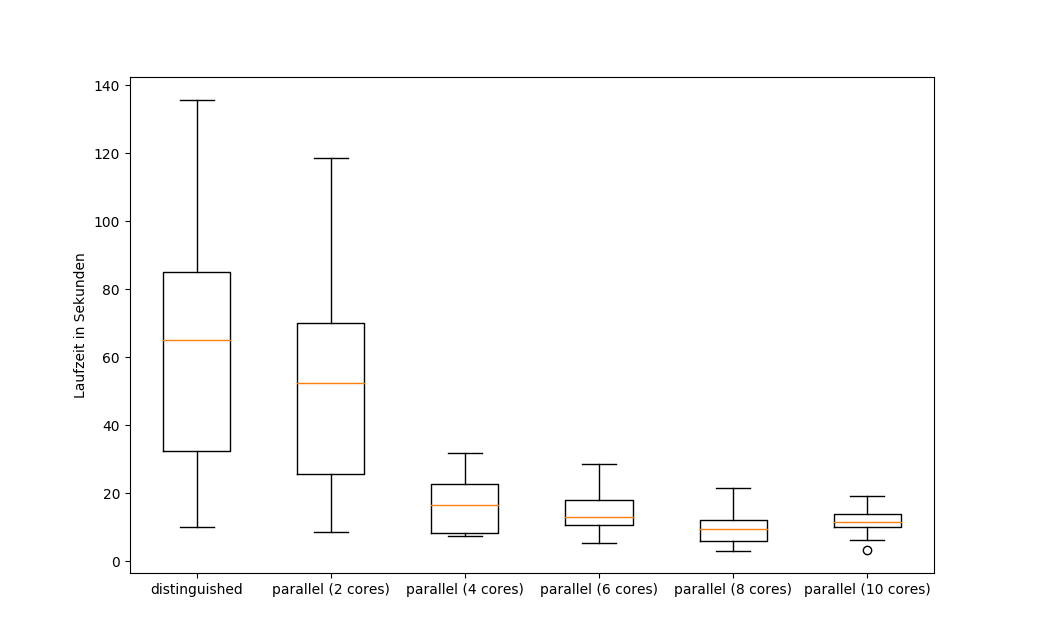
\includegraphics[width=0.75\textwidth]{../projekt/benchmark/plot_miserv_parallel.png}
  \caption{Grafische Darstellung der Rho-Methode in der Distinguished-Points-Variante ohne Parallelisierung, sowie parallelisiert mit 6 und 11 Threads}
  \label{fig:benchmark:parallel}
\end{figure}

\subsection{Rho Methode für das Faktorisieren}
\label{sec:rho_faktorisieren}
Die Rho Methode lässt sich generell auch für das Faktorisieren nutzen.
In unserer Implementierung haben wir dabei wieder die \emph{Floyd-Cycle} Suche genutzt.
Dies ist darin begründet, dass uns diese Zyklussuche als die am einfachsten
verständliche erschien.
In den von uns zur Berechnung verwendeten Größenordnungen haben wir den Nachteil in der
etwas längeren Laufzeit im Vergleich zu den anderen Zyklen als zu vernachlässigen
eingeschätzt.

Die implementierte Funktion lässt sich mit einem Parameter aufrufen.
Dies ist die zu faktorisierende Zahl.
Als Rückgabe erhält man einen Primfaktor dieser übergebenen Zahl.
Um weitere Primfaktoren zu erhalten muss die Rho Methode erneut gestartet werden.
Unsere Implementierung ist in \emph{rho\_faktorisieren.py} zu finden.

[schnellere Algorithmen: elliptic-curve factorization method (ECM), Quadratic sieve, General number field sieve]

\cite{Pollard1975}

\newpage
\printbibliography[heading=bibintoc]

\end{document}